\section{Regression Results for Individual Stocks}

The CAPM regression applied to individual stocks highlights significant findings regarding $\alpha$, $\beta$ and $R^2$ values 
(see Table~\ref{tab:regression_results} for reference).
Stocks like Johnson \& Johnson and Pfizer exhibit high $\beta$ coefficients, indicating a strong sensitivity to market
movements, with market returns explaining a substantial portion of their variability. These results confirm the applicability 
of the CAPM model to these stocks and its ability to estimate systematic risk effectively.
However, not all stocks perform equally well under the CAPM framework. Stocks like Cigna and Labcorp Holdings show relatively
low $R^2$ values, indicating that a smaller proportion of their return variability is explained by market factors. 
This suggests the presence of idiosyncratic risks or company-specific drivers that are not captured by the model. 
These discrepancies highlight the limitations of CAPM in explaining returns for stocks with unique business models or exposure 
to niche markets.
For stocks with lower $R^2$ values, alternative approaches, such as incorporating additional explanatory variables 
(e.g., size, value, or momentum factors), may enhance model reliability. 
These findings suggest that while the CAPM model provides a robust foundation for analyzing systematic risk, its assumptions
may need to be adjusted for certain stocks.

\begin{table}[htbp]
    \centering
    \footnotesize
    \renewcommand{\arraystretch}{1.2} % Adjust row height
    \begin{tabular}{|l|c|c|c|c|c|c|c|}
        \hline
        \rowcolor{unired!30} \textbf{Company} & \textbf{$\alpha$} & \textbf{$\beta$} & \textbf{$R^2$} & \textbf{Err. $\alpha$} & \textbf{Err. $\beta$} & \textbf{$\Delta \beta$ [0.025]} & \textbf{$\Delta \beta$ [0.975]} \\ \hline
        Johnson \& Johnson & 0.2451 & 0.7474 & 0.455 & 0.212 & 0.048 & 0.652 & 0.843 \\ \hline
        \rowcolor{gray!10} Boston Scientific & 0.3464 & 0.9036 & 0.207 & 0.458 & 0.105 & 0.698 & 1.109 \\ \hline
        Eli Lilly & 0.5655 & 0.9314 & 0.342 & 0.335 & 0.076 & 0.781 & 1.082 \\ \hline
        \rowcolor{gray!10} Pfizer & -0.3246 & 0.9595 & 0.451 & 0.274 & 0.063 & 0.836 & 1.083 \\ \hline
        Teleflex & 0.3055 & 0.9621 & 0.297 & 0.383 & 0.088 & 0.790 & 1.134 \\ \hline
        \rowcolor{gray!10} Cigna & 0.2511 & 1.0512 & 0.212 & 0.525 & 0.120 & 0.815 & 1.287 \\ \hline
        Revvity & -0.2457 & 1.2225 & 0.265 & 0.527 & 0.120 & 0.985 & 1.460 \\ \hline
        \rowcolor{gray!10} Medtronic & -0.1108 & 0.8613 & 0.384 & 0.282 & 0.065 & 0.734 & 0.988 \\ \hline
        LabCorp Holdings & 0.2675 & 0.9163 & 0.233 & 0.430 & 0.098 & 0.723 & 1.110 \\ \hline
        \rowcolor{gray!10} Humana & 0.5939 & 1.0700 & 0.231 & 0.506 & 0.116 & 0.843 & 1.298 \\ \Xhline{1.2\arrayrulewidth}

        \textbf{Portfolio} & \textbf{0.2234} & \textbf{0.8677} & \textbf{0.772} & \textbf{0.122} & \textbf{0.028} & \textbf{0.813 } & \textbf{0.923} \\ \hline
    \end{tabular}
    \caption{Regression results for each company, detailing Alpha, Beta, R-squared, and confidence intervals.}
    \label{tab:regression_results}
\end{table}

\section{Performance of the Weighted Portfolio}
The weighted portfolio demonstrates a strong alignment with the CAPM model, as evidenced by its significant and consistent
$\beta$ coefficient and high $R^2$ values. 
The compact and regular distribution of data points around the regression line highlights the effectiveness of diversification 
in reducing idiosyncratic risks and enhancing the model's explanatory power. 
This finding underscores the stability of portfolio returns when individual stock-specific risks are averaged out.
Compared to individual stocks, the portfolio benefits from a smoother relationship with market returns, as diversification 
minimizes the noise caused by unique company events. This results in more reliable estimates of $\beta$ and a higher goodness 
of fit ($R^2$), confirming the portfolio's sensitivity to systematic risk.
These characteristics make the CAPM model particularly suitable for analyzing aggregate portfolio behavior.
The portfolio's performance under the CAPM model reinforces the importance of diversification as a strategy for mitigating
risk and achieving more predictable returns. 
By averaging out the effects of outliers and company-specific shocks, the portfolio provides a clearer view of systematic 
risk and market sensitivity.

\begin{figure}[h]
    \centering
    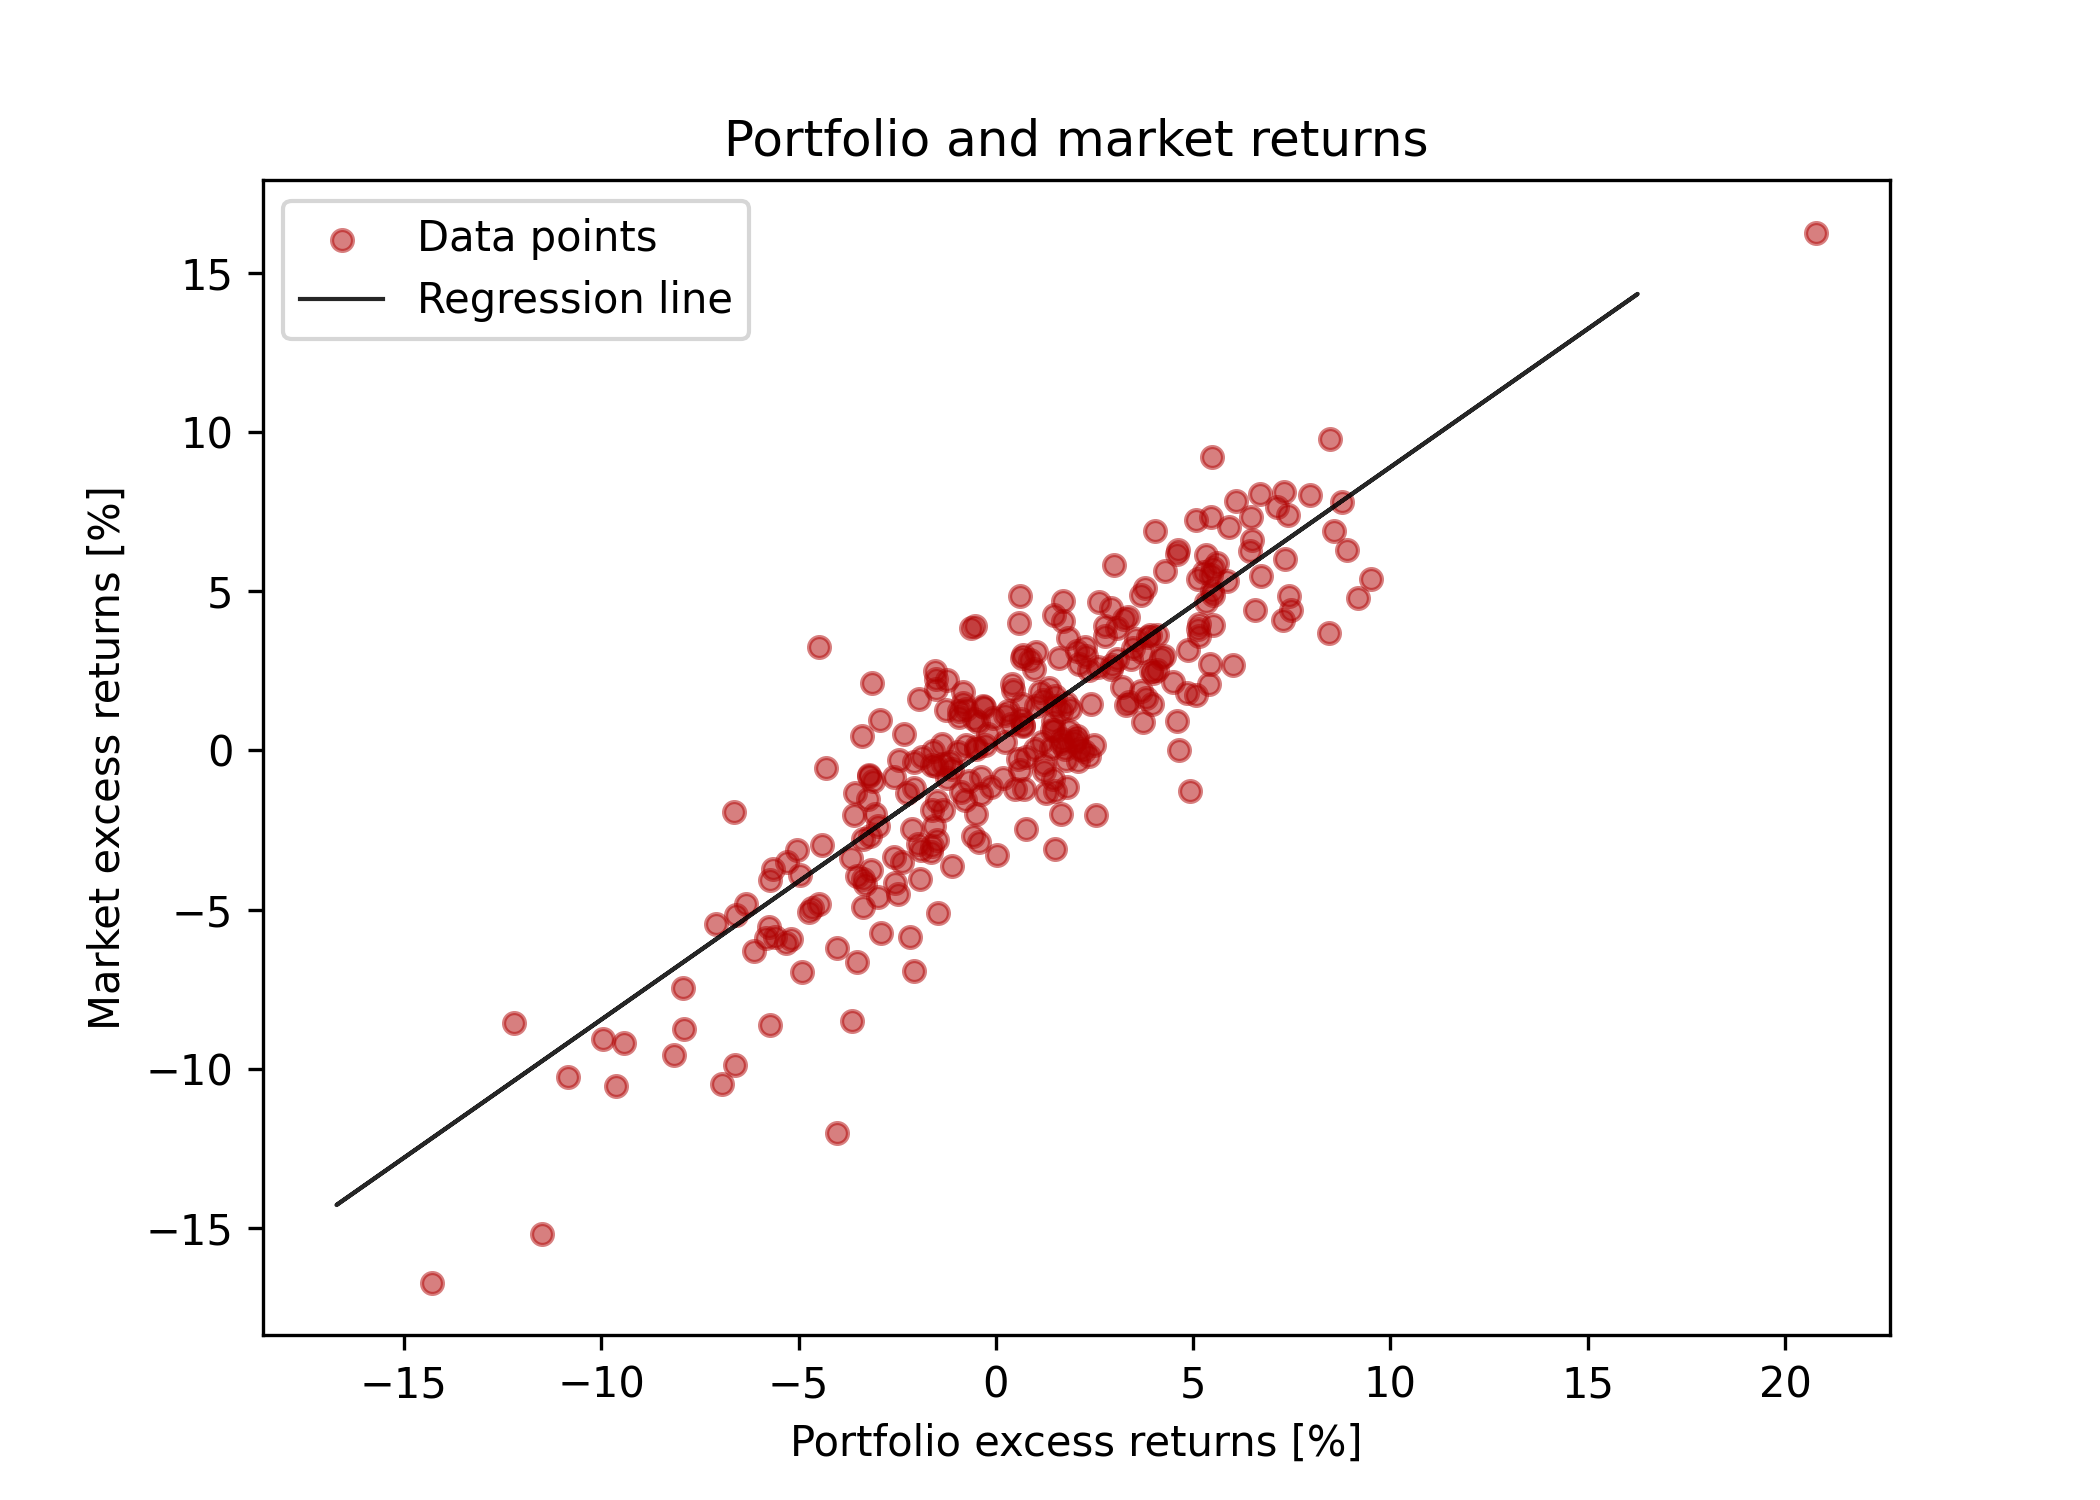
\includegraphics[width=0.8\textwidth]{images/portfolio_regression.png}
    \caption{Scatterplot of portfolio's returns against excess market returns, with linear regression.}\label{fig:portfolio_regression}
\end{figure}

\section{Impact of Diversification}
Diversification proves to be a key factor in stabilizing the parameter estimates of the CAPM model. 
While individual stocks may exhibit high variability in $\beta$ and $\alpha$ due to idiosyncratic risks, the equally weighted
portfolio achieves greater consistency. 
This is particularly evident in its reduced residual variance and higher $R^2$ values, which indicate a stronger fit to the 
CAPM framework.
The ability of diversification to average out company-specific risks highlights its role in improving the reliability of 
financial models. 
For investors, this suggests that constructing diversified portfolios can lead to more predictable risk and return profiles,
even when individual stocks deviate from expected patterns. 
Diversification also reduces the influence of outliers, providing a clearer picture of systematic risk.
These observations underscore the practical applications of the CAPM model for portfolio analysis, where diversification
enhances its explanatory power. 
However, the model's limitations in capturing unique factors for individual stocks emphasize the need for supplemental
analyses when evaluating less diversified assets.
